\section{Theorie}
\label{sec:Theorie}
In der Geometrischen Optik wird von Lichtstrahlen ausgegangen, die sich geradlinig im Raum ausbreiten.
Diese Lichtstrahlen können an einem optisch dichteren Medium gebrochen werden.
Bei dem Übergang in ein Anderes Medium wird ein Teil der Lichtstrahlen reflektiert und ein Teil erfährt eine
Richtungsänderung.
Als Medium werden Linsen betrachtet, dabei wird zwischen dünnen und dicken Sammellinsen und Zerstreuungslinsen
differenziert.
Eine dünne Sammellinse ist in Abbildung \ref{fig:dünn} d.argestellt
\begin{figure}
 \centering
 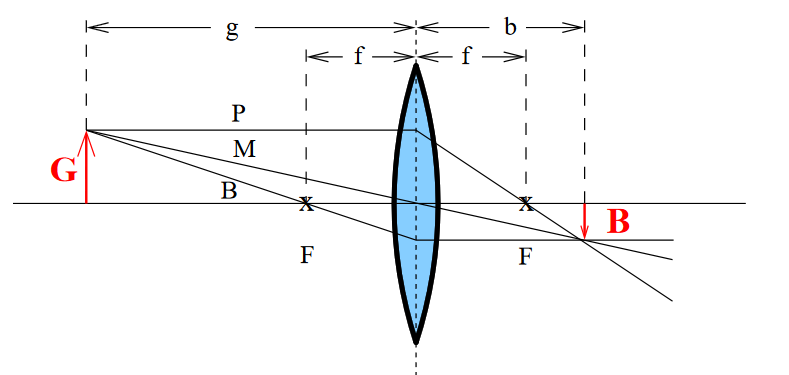
\includegraphics[width=0.7\textwidth]{dünn.png}
 \caption{Darstellung einer dünnen Linse.\cite{sample}}
 \label{fig:dünn}
 \end{figure}
 Die Sammellinse sammelt parallele Lichtstrahlen in dem Brennpunkt $F$.
